% Options for packages loaded elsewhere
\PassOptionsToPackage{unicode}{hyperref}
\PassOptionsToPackage{hyphens}{url}
%
\documentclass[
]{article}
\usepackage{amsmath,amssymb}
\usepackage{setspace}
\usepackage{iftex}
\ifPDFTeX
  \usepackage[T1]{fontenc}
  \usepackage[utf8]{inputenc}
  \usepackage{textcomp} % provide euro and other symbols
\else % if luatex or xetex
  \usepackage{unicode-math} % this also loads fontspec
  \defaultfontfeatures{Scale=MatchLowercase}
  \defaultfontfeatures[\rmfamily]{Ligatures=TeX,Scale=1}
\fi
\usepackage{lmodern}
\ifPDFTeX\else
  % xetex/luatex font selection
\fi
% Use upquote if available, for straight quotes in verbatim environments
\IfFileExists{upquote.sty}{\usepackage{upquote}}{}
\IfFileExists{microtype.sty}{% use microtype if available
  \usepackage[]{microtype}
  \UseMicrotypeSet[protrusion]{basicmath} % disable protrusion for tt fonts
}{}
\makeatletter
\@ifundefined{KOMAClassName}{% if non-KOMA class
  \IfFileExists{parskip.sty}{%
    \usepackage{parskip}
  }{% else
    \setlength{\parindent}{0pt}
    \setlength{\parskip}{6pt plus 2pt minus 1pt}}
}{% if KOMA class
  \KOMAoptions{parskip=half}}
\makeatother
\usepackage{xcolor}
\usepackage[margin=1.5in]{geometry}
\usepackage{color}
\usepackage{fancyvrb}
\newcommand{\VerbBar}{|}
\newcommand{\VERB}{\Verb[commandchars=\\\{\}]}
\DefineVerbatimEnvironment{Highlighting}{Verbatim}{commandchars=\\\{\}}
% Add ',fontsize=\small' for more characters per line
\usepackage{framed}
\definecolor{shadecolor}{RGB}{248,248,248}
\newenvironment{Shaded}{\begin{snugshade}}{\end{snugshade}}
\newcommand{\AlertTok}[1]{\textcolor[rgb]{0.94,0.16,0.16}{#1}}
\newcommand{\AnnotationTok}[1]{\textcolor[rgb]{0.56,0.35,0.01}{\textbf{\textit{#1}}}}
\newcommand{\AttributeTok}[1]{\textcolor[rgb]{0.13,0.29,0.53}{#1}}
\newcommand{\BaseNTok}[1]{\textcolor[rgb]{0.00,0.00,0.81}{#1}}
\newcommand{\BuiltInTok}[1]{#1}
\newcommand{\CharTok}[1]{\textcolor[rgb]{0.31,0.60,0.02}{#1}}
\newcommand{\CommentTok}[1]{\textcolor[rgb]{0.56,0.35,0.01}{\textit{#1}}}
\newcommand{\CommentVarTok}[1]{\textcolor[rgb]{0.56,0.35,0.01}{\textbf{\textit{#1}}}}
\newcommand{\ConstantTok}[1]{\textcolor[rgb]{0.56,0.35,0.01}{#1}}
\newcommand{\ControlFlowTok}[1]{\textcolor[rgb]{0.13,0.29,0.53}{\textbf{#1}}}
\newcommand{\DataTypeTok}[1]{\textcolor[rgb]{0.13,0.29,0.53}{#1}}
\newcommand{\DecValTok}[1]{\textcolor[rgb]{0.00,0.00,0.81}{#1}}
\newcommand{\DocumentationTok}[1]{\textcolor[rgb]{0.56,0.35,0.01}{\textbf{\textit{#1}}}}
\newcommand{\ErrorTok}[1]{\textcolor[rgb]{0.64,0.00,0.00}{\textbf{#1}}}
\newcommand{\ExtensionTok}[1]{#1}
\newcommand{\FloatTok}[1]{\textcolor[rgb]{0.00,0.00,0.81}{#1}}
\newcommand{\FunctionTok}[1]{\textcolor[rgb]{0.13,0.29,0.53}{\textbf{#1}}}
\newcommand{\ImportTok}[1]{#1}
\newcommand{\InformationTok}[1]{\textcolor[rgb]{0.56,0.35,0.01}{\textbf{\textit{#1}}}}
\newcommand{\KeywordTok}[1]{\textcolor[rgb]{0.13,0.29,0.53}{\textbf{#1}}}
\newcommand{\NormalTok}[1]{#1}
\newcommand{\OperatorTok}[1]{\textcolor[rgb]{0.81,0.36,0.00}{\textbf{#1}}}
\newcommand{\OtherTok}[1]{\textcolor[rgb]{0.56,0.35,0.01}{#1}}
\newcommand{\PreprocessorTok}[1]{\textcolor[rgb]{0.56,0.35,0.01}{\textit{#1}}}
\newcommand{\RegionMarkerTok}[1]{#1}
\newcommand{\SpecialCharTok}[1]{\textcolor[rgb]{0.81,0.36,0.00}{\textbf{#1}}}
\newcommand{\SpecialStringTok}[1]{\textcolor[rgb]{0.31,0.60,0.02}{#1}}
\newcommand{\StringTok}[1]{\textcolor[rgb]{0.31,0.60,0.02}{#1}}
\newcommand{\VariableTok}[1]{\textcolor[rgb]{0.00,0.00,0.00}{#1}}
\newcommand{\VerbatimStringTok}[1]{\textcolor[rgb]{0.31,0.60,0.02}{#1}}
\newcommand{\WarningTok}[1]{\textcolor[rgb]{0.56,0.35,0.01}{\textbf{\textit{#1}}}}
\usepackage{graphicx}
\makeatletter
\def\maxwidth{\ifdim\Gin@nat@width>\linewidth\linewidth\else\Gin@nat@width\fi}
\def\maxheight{\ifdim\Gin@nat@height>\textheight\textheight\else\Gin@nat@height\fi}
\makeatother
% Scale images if necessary, so that they will not overflow the page
% margins by default, and it is still possible to overwrite the defaults
% using explicit options in \includegraphics[width, height, ...]{}
\setkeys{Gin}{width=\maxwidth,height=\maxheight,keepaspectratio}
% Set default figure placement to htbp
\makeatletter
\def\fps@figure{htbp}
\makeatother
\setlength{\emergencystretch}{3em} % prevent overfull lines
\providecommand{\tightlist}{%
  \setlength{\itemsep}{0pt}\setlength{\parskip}{0pt}}
\setcounter{secnumdepth}{5}
\newlength{\cslhangindent}
\setlength{\cslhangindent}{1.5em}
\newlength{\csllabelwidth}
\setlength{\csllabelwidth}{3em}
\newlength{\cslentryspacingunit} % times entry-spacing
\setlength{\cslentryspacingunit}{\parskip}
\newenvironment{CSLReferences}[2] % #1 hanging-ident, #2 entry spacing
 {% don't indent paragraphs
  \setlength{\parindent}{0pt}
  % turn on hanging indent if param 1 is 1
  \ifodd #1
  \let\oldpar\par
  \def\par{\hangindent=\cslhangindent\oldpar}
  \fi
  % set entry spacing
  \setlength{\parskip}{#2\cslentryspacingunit}
 }%
 {}
\usepackage{calc}
\newcommand{\CSLBlock}[1]{#1\hfill\break}
\newcommand{\CSLLeftMargin}[1]{\parbox[t]{\csllabelwidth}{#1}}
\newcommand{\CSLRightInline}[1]{\parbox[t]{\linewidth - \csllabelwidth}{#1}\break}
\newcommand{\CSLIndent}[1]{\hspace{\cslhangindent}#1}
\ifLuaTeX
\usepackage[bidi=basic]{babel}
\else
\usepackage[bidi=default]{babel}
\fi
\babelprovide[main,import]{italian}
% get rid of language-specific shorthands (see #6817):
\let\LanguageShortHands\languageshorthands
\def\languageshorthands#1{}
\ifLuaTeX
  \usepackage{selnolig}  % disable illegal ligatures
\fi
\IfFileExists{bookmark.sty}{\usepackage{bookmark}}{\usepackage{hyperref}}
\IfFileExists{xurl.sty}{\usepackage{xurl}}{} % add URL line breaks if available
\urlstyle{same}
\hypersetup{
  pdftitle={FASI DI CRESCITA DI UNA PIANTA},
  pdfauthor={Alessia Raio},
  pdflang={it},
  hidelinks,
  pdfcreator={LaTeX via pandoc}}

\title{FASI DI CRESCITA DI UNA PIANTA}
\usepackage{etoolbox}
\makeatletter
\providecommand{\subtitle}[1]{% add subtitle to \maketitle
  \apptocmd{\@title}{\par {\large #1 \par}}{}{}
}
\makeatother
\subtitle{le fasi della crescita delle piante}
\author{Alessia Raio}
\date{}

\begin{document}
\maketitle

{
\setcounter{tocdepth}{3}
\tableofcontents
}
\setstretch{0.5}
\begin{verbatim}
##   weight group
## 1   4.17  ctrl
## 2   5.58  ctrl
## 3   5.18  ctrl
## 4   6.11  ctrl
## 5   4.50  ctrl
## 6   4.61  ctrl
\end{verbatim}

\begin{Shaded}
\begin{Highlighting}[]
\FunctionTok{summary}\NormalTok{(dati)}
\end{Highlighting}
\end{Shaded}

\begin{verbatim}
NA      weight       group   
NA  Min.   :3.590   ctrl:10  
NA  1st Qu.:4.550   trt1:10  
NA  Median :5.155   trt2:10  
NA  Mean   :5.073            
NA  3rd Qu.:5.530            
NA  Max.   :6.310
\end{verbatim}

\includegraphics{prova_files/figure-latex/unnamed-chunk-3-1.pdf}

\begin{Shaded}
\begin{Highlighting}[]
\FunctionTok{plot}\NormalTok{(dati}\SpecialCharTok{$}\NormalTok{y }\SpecialCharTok{\textasciitilde{}}\NormalTok{ dati}\SpecialCharTok{$}\NormalTok{x)}
\end{Highlighting}
\end{Shaded}

\begin{Shaded}
\begin{Highlighting}[]
\NormalTok{PlantGrowth}
\end{Highlighting}
\end{Shaded}

\begin{verbatim}
     weight group
  1    4.17  ctrl
  2    5.58  ctrl
  3    5.18  ctrl
  4    6.11  ctrl
  5    4.50  ctrl
  6    4.61  ctrl
  7    5.17  ctrl
  8    4.53  ctrl
  9    5.33  ctrl
....
\end{verbatim}

\begin{Shaded}
\begin{Highlighting}[]
\NormalTok{knitr}\SpecialCharTok{::}\FunctionTok{include\_graphics}\NormalTok{(}\AttributeTok{path =} \StringTok{"immagini/piante.jpg"}\NormalTok{)}
\end{Highlighting}
\end{Shaded}

\begin{figure}

{\centering 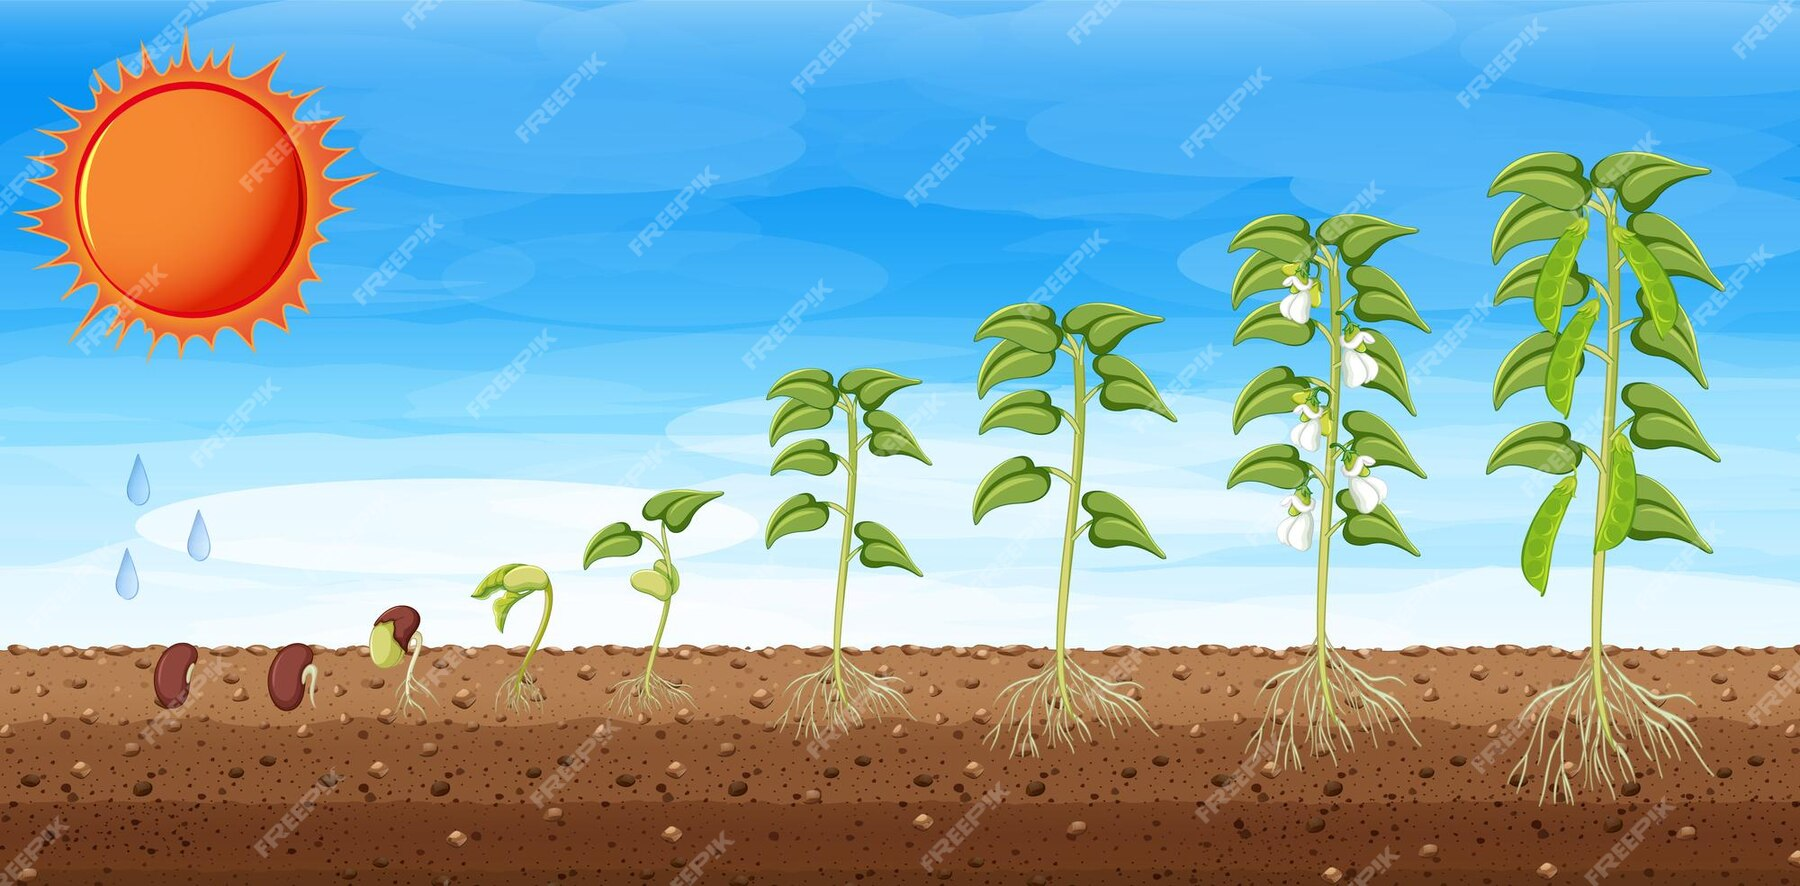
\includegraphics[width=0.5\linewidth]{immagini/piante} 

}

\caption{fasi di crescita di una piantina}\label{fig:unnamed-chunk-6}
\end{figure}

\hypertarget{introduzione}{%
\section{Introduzione}\label{introduzione}}

\href{https://it.wikipedia.org/wiki/Ky\%C5\%ABjitai}{\color{red}{Kyūjitai}\normalcolor}

\textbf{Le piante} hanno una vita molto simile alla nostra. Anche loro
passano attraverso diverse fasi di crescita, a partire dalla
germinazione fino alla senescenza. A differenza nostra, però, le piante
presentano una vita ciclica che si ripete di stagione in stagione.

\hypertarget{pianto}{%
\section{Pianto}\label{pianto}}

In questa fase così affascinante da osservare, si riattiva il
\textbf{metabolismo} della pianta e la respirazione cellulare. La linfa
vitale sale dalle radici fino alle foglie, passando dai tralci. Dai
tagli effettuati durante la potatura escono piccole gocce di linfa
simili a lacrime (da cui il nome pianto della vite) in quantità che va
\textbf{\emph{da pochi decilitri a qualche litro per pianta.}}

\begin{quote}
Questo processo dura 15-20 giorni e avviene tra la fine di marzo e i
primi di aprile.
\end{quote}

\hypertarget{germogliamento}{%
\section{Germogliamento}\label{germogliamento}}

Si tratta del momento di schiusura delle gemme.

Questa fase inizia 2 o 3 giorni dopo l'inizio del pianto, quindi tra
fine marzo (nelle zone più a sud) e i primi di aprile (al centro e al
nord).

Affinchè inizi ci devono essere alcune condizioni tra cui una
temperatura intorno ai \color{red}{7-12°C.} \normalcolor

La crescita dei germogli è massima durante la fioritura.

\begin{figure}
\centering
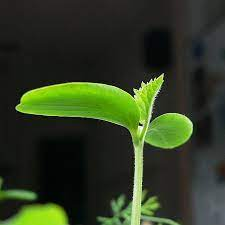
\includegraphics{immagini/germ.jpeg}
\caption{germoglio}
\end{figure}

\hypertarget{fioritura}{%
\section{Fioritura}\label{fioritura}}

\textbf{La formazione dei fiori} avviene fra la fine di aprile e
l'inizio di giugno, a seconda della
latitudine.\color{green}{Lorem ipsum} \normalcolor I fiori della vite
sono poco appariscenti ed hanno la forma di una piccola pannocchia
verde. Sono ermafroditi e l'impollinazione è anemofila, ossia avviene
grazie al trasporto del polline da parte del vento, non necessita degli
insetti.

Dai fiori fecondati (che sonodal 30 al 60\% dei fiori totali, in base al
vitigno) si sviluppano quelli che saranno acini, i fiori non fecondati
invece muoiono e cadono.

dolor sit amet, consectetur adipiscing elit. Cras mauris turpis,
convallis quis mauris vel, volutpat dapibus sapien. Ut convallis, nisi
id scelerisque tristique, tortor massa tincidunt purus, ut pellentesque
turpis mi eu velit. Ut ac lectus at ligula pellentesque egestas id eu
urna. In eu tristique mauris. Ut ut lacus velit. Nullam eget molestie
urna, eget tempor odio. Duis et ante et lorem porttitor molestie. In dui
diam, iaculis sed erat non, suscipit imperdiet risus. Proin bibendum
viverra gravida. Nulla venenatis risus in felis rhoncus pretium in quis
odio. Suspendisse potenti. Sed condimentum interdum metus, sit amet
vestibulum mauris vestibulum at. Morbi non orci at augue dapibus
tristique non eget ipsum. Morbi elementum nunc non odio elementum
elementum. (Epifania, Anselmi, e Robusto 2020)

\color{blue}{Vivamus eleifend sollicitudin libero vitae maximus}\normalcolor.
In lobortis justo non commodo auctor. Integer suscipit ipsum non ipsum
rhoncus, quis posuere velit interdum. Praesent nec dictum libero, vel
imperdiet arcu. Aenean vel gravida sem. Fusce dictum lectus a mollis
vehicula. Aenean vel euismod libero, vel suscipit enim. Aenean et nulla
finibus, egestas dolor quis, vestibulum arcu. Suspendisse facilisis enim
quis eros ullamcorper mollis. Donec porttitor vulputate mi, id finibus
urna fermentum quis. Nam tincidunt sem eu tempor consectetur.
Suspendisse in luctus erat. Morbi suscipit pulvinar malesuada. Ut
bibendum turpis sed ultrices sagittis. Vestibulum quam tortor, egestas
at mollis ac, tempor id velit. Morbi vitae elementum quam\footnote{lorem}.
(Epifania, Anselmi, e Robusto 2021)

\begin{itemize}
\tightlist
\item
  guerra

  \begin{itemize}
  \tightlist
  \item
    giappone
  \item
    lorem
  \end{itemize}
\item
  ipsum
\end{itemize}

\begin{enumerate}
\def\labelenumi{\arabic{enumi}.}
\tightlist
\item
  marina\footnote{militare}
\item
  militare
\item
  giapponese
\item
  in guerra
\end{enumerate}

\begin{table}[!htbp] \centering 
  \caption{Tabella di summary} 
  \label{} 
\begin{tabular}{@{\extracolsep{5pt}}lccccc} 
\\[-1.8ex]\hline 
\hline \\[-1.8ex] 
Statistic & \multicolumn{1}{c}{N} & \multicolumn{1}{c}{Mean} & \multicolumn{1}{c}{St. Dev.} & \multicolumn{1}{c}{Min} & \multicolumn{1}{c}{Max} \\ 
\hline \\[-1.8ex] 
weight & 30 & 5.07 & 0.70 & 3.59 & 6.31 \\ 
\hline \\[-1.8ex] 
\end{tabular} 
\end{table}

\begin{table}[!htbp] \centering 
  \caption{Risultati del modello} 
  \label{} 
\begin{tabular}{@{\extracolsep{5pt}}lc} 
\\[-1.8ex]\hline 
\hline \\[-1.8ex] 
 & \multicolumn{1}{c}{\textit{Dependent variable:}} \\ 
\cline{2-2} 
\\[-1.8ex] & y \\ 
\hline \\[-1.8ex] 
 xtrt1 & $-$0.37 \\ 
  & (0.28) \\ 
  & \\ 
 xtrt2 & 0.49$^{*}$ \\ 
  & (0.28) \\ 
  & \\ 
 Constant & 5.03$^{***}$ \\ 
  & (0.20) \\ 
  & \\ 
\hline \\[-1.8ex] 
Observations & 30 \\ 
R$^{2}$ & 0.26 \\ 
Adjusted R$^{2}$ & 0.21 \\ 
Residual Std. Error & 0.62 (df = 27) \\ 
F Statistic & 4.85$^{**}$ (df = 2; 27) \\ 
\hline 
\hline \\[-1.8ex] 
\textit{Note:}  & \multicolumn{1}{r}{$^{*}$p$<$0.1; $^{**}$p$<$0.05; $^{***}$p$<$0.01} \\ 
\end{tabular} 
\end{table}

\begin{Shaded}
\begin{Highlighting}[]
\NormalTok{ m0 }\OtherTok{=} \FunctionTok{lm}\NormalTok{(y }\SpecialCharTok{\textasciitilde{}}\NormalTok{ x, }\AttributeTok{data =}\NormalTok{ dati)}
\NormalTok{ m1 }\OtherTok{=} \FunctionTok{lm}\NormalTok{(y }\SpecialCharTok{\textasciitilde{}}\NormalTok{ x, }\AttributeTok{data =}\NormalTok{ dati)}
 \FunctionTok{stargazer}\NormalTok{(m0, m1, }\AttributeTok{type =} \StringTok{"latex"}\NormalTok{, }\AttributeTok{title =} \StringTok{"Model comparison"}\NormalTok{, }\AttributeTok{digits =} \DecValTok{2}\NormalTok{, }\AttributeTok{intercept.top =} \ConstantTok{TRUE}\NormalTok{,}
     \AttributeTok{intercept.bottom =} \ConstantTok{FALSE}\NormalTok{, }\AttributeTok{header =} \ConstantTok{FALSE}\NormalTok{)}
\end{Highlighting}
\end{Shaded}

\begin{table}[!htbp] \centering 
  \caption{Model comparison} 
  \label{} 
\begin{tabular}{@{\extracolsep{5pt}}lcc} 
\\[-1.8ex]\hline 
\hline \\[-1.8ex] 
 & \multicolumn{2}{c}{\textit{Dependent variable:}} \\ 
\cline{2-3} 
\\[-1.8ex] & \multicolumn{2}{c}{y} \\ 
\\[-1.8ex] & (1) & (2)\\ 
\hline \\[-1.8ex] 
 Constant & 5.03$^{***}$ & 5.03$^{***}$ \\ 
  & (0.20) & (0.20) \\ 
  & & \\ 
 xtrt1 & $-$0.37 & $-$0.37 \\ 
  & (0.28) & (0.28) \\ 
  & & \\ 
 xtrt2 & 0.49$^{*}$ & 0.49$^{*}$ \\ 
  & (0.28) & (0.28) \\ 
  & & \\ 
\hline \\[-1.8ex] 
Observations & 30 & 30 \\ 
R$^{2}$ & 0.26 & 0.26 \\ 
Adjusted R$^{2}$ & 0.21 & 0.21 \\ 
Residual Std. Error (df = 27) & 0.62 & 0.62 \\ 
F Statistic (df = 2; 27) & 4.85$^{**}$ & 4.85$^{**}$ \\ 
\hline 
\hline \\[-1.8ex] 
\textit{Note:}  & \multicolumn{2}{r}{$^{*}$p$<$0.1; $^{**}$p$<$0.05; $^{***}$p$<$0.01} \\ 
\end{tabular} 
\end{table}

\[z_i = \dfrac{x_i - \bar{x} }{sd}\]
\[z_i = `r{\dfrac{((dati$y[1]) - \(mean(dati$y)))}{sd(dati$y)}}` \]

\newpage

\hypertarget{references}{%
\section*{References}\label{references}}
\addcontentsline{toc}{section}{References}

\hypertarget{refs}{}
\begin{CSLReferences}{1}{0}
\leavevmode\vadjust pre{\hypertarget{ref-epifania2020dscoreapp}{}}%
Epifania, Ottavia M, Pasquale Anselmi, e Egidio Robusto. 2020.
{«Dscoreapp: A shiny web application for the computation of the implicit
association test d-score»}. \emph{Frontiers in Psychology} 10: 489006.

\leavevmode\vadjust pre{\hypertarget{ref-epifania2021implicit}{}}%
---------. 2021. {«Implicit social cognition through the years: The
Implicit Association Test at age 21.»} \emph{Psychology of
Consciousness: Theory, Research, and Practice}.
https://doi.org/\url{https://doi.org/10.1037/cns0000305}.

\end{CSLReferences}

\end{document}
